\section{Introducción}

En el presente trabajo se busca modelar y resolver el problema de determinar un orden de importancia de las páginas webs. El mismo es utilizado por motores de búsqueda como un factor determinante a la hora de arrojar resultados que se intentan que sean los más aproximados a lo que se pretende encontrar en la red de redes.

Varios criterios para la confección de un ranking pueden establecerse (como tráfico promedio, correspondencias entre nombres o descripciones de la web y lo que se deas buscar, etc) pero solo nos concentraremos en uno: PageRank.  \\

\subsection{PageRank}

Este método cuyo nombre deriva de su diseñador y a su vez confundador de Google, Larry Page, pone su atención en los enlaces entre páginas pertenencientes a un conjunto de páginias presuntamente relacionadas por la tématica que el usuario busca.\\

Modelandolo mátematicamente, se puede pensar pensar a cada una de las páginas como un vértice y los links entre ellas como ejes dirigidos. De esta menera generamos un grafo dirigido como el que se muestra a continuación:   

\begin{figure}[H]
   \begin{center}
     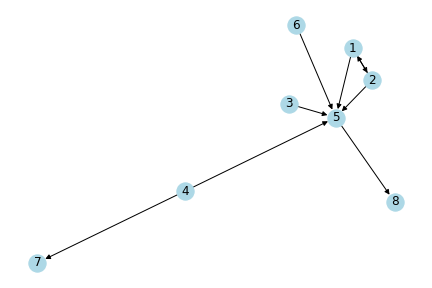
\includegraphics{img/ejemplo.png} 
  \end{center}
\caption{Ejemplo de grafo dirigido de páginas webs.} \label{fig:ejemplo}
\end{figure}

El grafo es simple ya que se descartan los autolinks que puedan existir con el fin de no sobrevalorar artificialmente a cada nodo.\\

Como tomamos en cuenta los enlnaces a la hora, el ranking más sencillo que se puede obtener a partir de un grafo de páginas es simplemente contar el grado de salida de cada nodo y ordenar a cada vértice según dicho resultado. En teoría de grafos se define grado de salida de un nodo $v$ como la cantidad de ejes dirigidos, notados matemáticamente como el par ordenado $(v,w)$, que van desde $v$ a otro nodo $w$ del grafo. Grado de entrado es lo mismo pero contanod los ejes que se reciben. 
\\

En en nuestro ejemplo la página mejor rankeada es la 5, ya que cuenta con 5 ejes de entrada. Surge la pregunta de si este es un ranking criterioso. En el mundo real no es lo mismo que a una página la apunte una reconocida mundialmente y con un tráfico de usuarios del orden de millones por día que una de decenas de visitas diarias y de reconocimiento local. Este es un problema que el criterio sencillo planteado anteriormente no puede resolver.
Alternativamente, si ordenamos por grado de salida encontramos que las páginas 1,2 y 4 son las mejores rankeadas. Sin embargo, esto sobreestima aquellas webs que son indexadoras por sobre las autoritativas en un tópico deseado.\\

PageRank, en cambio, pondera los enlaces que recibe una página. El puntaje asignado a cada una no solo depende de la cantidad de links recibidos sino también del puntaje de esas páginas que la apuntan. De esta manera se trata de medir la calidad de los ejes teniendo en cuenta la importancia del nodo enlacador en relación a la red analizada.\\

Formalmente, definimos W como la matriz transpuesta de lo que en teoría de Grafos se conoce como mátriz de adyacencia.
Se busca distribuir los enlaces en la misma por lo que su dimensión es de $cantidad de nodos \times cantida de nodos$.

$w_{i,j} = 1$ sii existe un arco $(j,i)$ en el grafo, es decir, un link de la página $j$ a la página $i$. Caso contrario la entrada vale 0. Notar que en cada fila $i$, las entradas con valor 1 indican las páginas que apuntan a la página $i$. Por lo que $\sum_{j=1}^{n} w_{i,j}$ = $grado_{in} i$. Así como la suma de la fila i representa el grado de entrada de dicha fila, la suma de las columnas representa el grado de salida (que denominamos $c_{i}$) y por lo tanto la cantidad de links salientes de la misma. \\

El método de PageRank define el aporte que otorga un enlace de una página $j$ a una página $i$ como $\frac{x_{j}}{c_{j}} w_{ij}$ , donde $x_{j}$ es el puntaje de la página $j$. Notar que si no hay link, el aporte es nulo.
El puntaje por su parte se define como $x_{j}$ = $\sum_{k=1}^{n} aporte (w_{j,k})$. De esta manera el armado del ranking toma en cuenta la calidad del eje al ponderar el enlace por el puntaje del enlazador sobre la cantida de nodos a los que les distribuye su puntaje ($g_{out} j$). De esta manera se busca que no valga lo mismo un link proveniente de un página con mucho puntaje que uno proveniente de una págian con poco puntaje. A su vez, el puntaje de un nodo es distribuido equitativamente entre todos los enlaces salientes del mismo, razon por la cual se divide el puntaje por el grado de salida en el aporte de un link. \\ \\

La matriz W del ejemplo es la siguiente: W = 
$ \begin{pmatrix}
  0 & 1 & 0 & 0 & 0 & 0 & 0 & 0 \\
 1 & 0 & 0 & 0 & 0 & 0 & 0 & 0  \\
  0 & 0 & 0 & 0 & 0 & 0 & 0 & 0  \\
   0 & 0 & 0 & 0 & 0 & 0 & 0 & 0  \\
    1 & 1 & 1 & 1 & 0 & 1 & 0 & 0  \\
     0 & 0 & 0 & 0 & 0 & 0 & 0 & 0  \\
      0 & 0 & 0 & 1 & 0 & 0 & 0 & 0  \\
       0 & 0 & 0 & 0 & 1 & 0 & 0 & 0  \\
 \end{pmatrix}$ \\ \\ 
 
 Definimos la matriz diagonal D, con     
    \begin{equation*}
        d_{jj} = \left\{
                \begin{array}{ll}
                     1/cj & \mathrm{si\ } c_j \neq 0 \\
                     0    & \mathrm{si\ } c_j = 0
                \end{array}
            \right.
    \end{equation*} 

Si multiplicamos $WD$ = $R$ obtenemos una matriz donde cada link es divido por el grado de salida del nodo apuntador. En el caso del ejemplo, R es: \\ \\



$ \begin{pmatrix}
  0 & 1/2 & 0 & 0 & 0 & 0 & 0 & 0 \\
 1/2 & 0 & 0 & 0 & 0 & 0 & 0 & 0  \\
  0 & 0 & 0 & 0 & 0 & 0 & 0 & 0  \\
   0 & 0 & 0 & 0 & 0 & 0 & 0 & 0  \\
    1/2 & 1/2 & 1 & 1/2 & 0 & 1 & 0 & 0  \\
     0 & 0 & 0 & 0 & 0 & 0 & 0 & 0  \\
      0 & 0 & 0 & 1/2 & 0 & 0 & 0 & 0  \\
       0 & 0 & 0 & 0 & 1 & 0 & 0 & 0  \\
 \end{pmatrix}$ \\ \\


Resolviendo el sistema de ecuaciones $Rx$ = $x$ obtenemos el ranking de PageRank ya que en la posición $x_{i}$ = $fila_{i} R$x = $\sum_{j=1}^{n} aporte (w_{i,j})$. Al resultado se lo normaliza para que sea un vector de probabilidad. \\

Ahora bien, este modelo no contempla el caso en el que las páginas no tienen links salientes como la red del ejemplo. 

\subsubsection{Navegante Aleatorio}

Para resolver este problema se propone un modelo en el cual un navegante recorre la red pasando de una página a otra vecina con una probabilidad $p$ y a otra cualquiera del grafo con una probabilidad $1-p$. Si la página no contiene links de salidas entonces el navegante elige al azar cualquier página. De este modo no se queda estancado en un nodo sin links saliente sino que puede elegir una cualquiera con cierta probabilidad. Se inenta modelar así el comportamiento de un unsuario de Internet donde no solo viaje de página en página a traves de links de estas sino que también puede escribir la url de la misma o acceder por marcadores. \\

Ahora la matriz que llamamos A $\in \mathbb{R}^{n \times n}$, donde $n$ es la cantidad de páginas, contiene en cada posición $ij$ la probabilidad de de pasar de la página j a la i estando en j. Matemáticamente se define por la siguiente ecuación:

    \begin{equation}
        a_{ij} = \left\{
                \begin{array}{ll}
                     (1-p)/n + p w_{ij}/c_{j} & \mathrm{si\ } c_j \neq 0 \\
                     1/n    & \mathrm{si\ } c_j = 0
                \end{array}
            \right.
    \end{equation} 

A diferencia de antes, ahora contemplamos una probabilidad de seguir por la estructura del grafo y otra de no hacerlo. Por lo tanto el ranking está determinado por la suma ponderada no solo por la importancia de la páginas enlazadoras sino tambien por dicha probabilidad. Luego el puntaje $x_{i}$ de la página $i$ es igual a $\sum_{j=1}^{n} a_{ij} * aporte (w_{i,j})$ y para ello se debe resovler el sistema de ecuaciones $Ax$ = $x$, con $p$ $\in$ (0,1) y vector x normalizado.\\

En la siguiente sección del presente trabajo se demuestra la equivalencia entre este sitema de ecuaciones y otro que efectivamente resolvemos para calcular el ranking. Dicho sistema pueden resolverse haciendo uso de elementos del Álgebra Lineal que indtroducimos brevemente a continuación. \\

En el caso de nuestro ejemplo, si tomamos p = 0.85 el raking es[0.0998393 ,0.0998393 ,0.0574076 ,0.0574076 ,0.264262 ,0.0574076,0.0818058 ,0.28203 ]. Notar que el nodo más apuntado (el 5) no es el de mayor puntaje. \\

\subsection{Sistemas de ecuaciones lineales y Eliminación Gaussiana}

Un sistema de ecuaciones lineales de n incognitas ($x_{1} \dots x_{n}$) y n ecuaciones se define del siguiente modo:

    \begin{equation*}
     	\left\{
                \begin{array}{l}
                
                     a_{1,1}x_{1} + a_{1,2}x_{2} + \dots + a_{1,n}x_{n} =  b_{1} \\
                     \vdots \\ 
                    a_{n,1}x_{1} + a_{n,2}x_{2} + \dots + a_{n,n}x_{n} =  b_{n} 
                    
                \end{array}
       \right.
    \end{equation*}  
    
Queremos resolver Ax = b, donde $a_{ij}$ es el coeficiente de la ecuación $i$ que multiplica a la varaible $x_{j}$. Para ello contamos con el método de Eliminación Gaussiana \cite{burden}. 
Se itera $n$ veces y en cada iteración se realiza el siguiente cálculo: 
$a_{ij}$ = $a_{ij}$ $-$ $\frac{a_{ik}}{a_{kk}} a_{kj}$  con $k < i,j \leq n$, siendo k la k-ésima iteración.
Lo mismo ocurre para el $b$. $b_{i}$ = $b_{i}$ $-$ $\frac{a_{ik}}{a_{kk}} b_{k}$ \\
Esto triangula la matriz quedando una columna de ceros debajo de cada diagonal. La matriz resultante es entonces triangular superior de la siguiente pinta: \\ \\

$\begin{pmatrix}
a_{11} & \dots & a_{1n} \\
0 & a_{22}^{(1)} & \dots & a_{2n}^(1) \\
\vdots &  & \ddots  & \vdots \\
0 & \dots & & a_{nn}^(n)       \\
\end{pmatrix}$ \\ \\

Con algún $b^{'}$. Esto vale siempre que el pivot escogido, el $a_{kk}^(k)$ sea no nulo. En la sección de desarrollo demostramos que para el caso de las matrices que debemos resolver en este trabajo se cumple esta condición.\\

Una vez obtenida la matriz triangular superior se despejan las incógnitas con backward-substitution. Comenzando por la última variable $x_{n}$, se despeja para arriba siendo $x_{i}$ = $b_{i} - \sum_{j=i+1}^{n} a_{ij}x_{j}$. Como el despeje es de n hasta 1 nos aseguramos de contar con la variables siguientes $x_{i}$ ya calculadas. 
La complejidad temporal de Eliminación Gaussiana es cúbica en función de $n$ (filas de la matriz), mientras que la de backward substitution es cuadrática. En total entonces, asintóticamente, el requerimiento computación temporal de la resolución de un sistema de ecuaciones lineales es cúbico.\\

\subsection{Matriz rala}

Se denomina matriz rala a una matriz con muchos elementos nulos. Dado que una red de la web la mayoría de las páginas no poseen demasiados links de entrada o de salida (seguramente una página enlace a pocas salvo que sea un indexador), las matrices con las que trabajaremos son poco densas. Debido a esto, buscamos optimizar el almacenamiento de la misma e intentar acelerar los cálculos lo más rápido que se pueda al asegurarnos de almacenar solo los elementos no nulos y modificar la eliminación Gaussiana de manera que aproveche tal estrucutra de datos. 
En la siguiente sección se detalla la implementación escogida para este trabajo.\\ \\

En la sección desarrollo Desarrollo se demuestran algunas propiedas del sistema a resolver, como la equivalencia entre el mismo y el introducido en la presente exposición preliminar, la posibilidad de realización de la Eliminación Gaussiana y luego se detalla la implementación utilizada.\\

En la sección siguiente se aborda la experimentación llevada a cabo. Se exponen los objetivos tanto de los test cuantitativos como cualitativos, hipótesis acerca del resultado de los mismos y luego se muestran lo más ilustrativamente posible lo que arrojaron tales experiencias. Un análisis profundo y pertinente le sigue a cada una. \\

Por último se expone lo concluido de este trabajo, haciendo un fuerte énfasis en lo observado empíricamente, relacionándolo con los conocimientos que tenemos de la formulación matemática del modelo de PageRank, sus cualidades y características como ranking de páginas webs y posibles extensiones de su uso.




 